\documentclass{beamer}
\usetheme{Madrid}

\usepackage{ctex}
\usepackage{tikz}

\newcommand{\concept}[1]{{\color{blue} #1}}

\newcommand{\Ga}{\alpha}
\newcommand{\Gb}{\beta}
\newcommand{\Gg}{\gamma}     \newcommand{\GG}{\Gamma}
\newcommand{\Gd}{\delta}     \newcommand{\GD}{\Delta}
\newcommand{\Ge}{\epsilon}
\newcommand{\Gf}{\phi}       \newcommand{\GF}{\Phi}
\newcommand{\Gh}{\theta}
\newcommand{\Gi}{\iota}
\newcommand{\Gk}{\kappa}
\newcommand{\Gl}{\lambda}    \newcommand{\GL}{\Lambda}
\newcommand{\Go}{\omega}     \newcommand{\GO}{\Omega}
\newcommand{\Gs}{\sigma}
\newcommand{\Gt}{\tau}
\newcommand{\Gz}{\zeta}

\title{EM 算法}
\author{祝润天}
\institute{复旦大学计算机科学技术学院}
\date{2024 年 12 月 6 日}

\begin{document}

\begin{frame}
    
    \maketitle

\end{frame}

\begin{frame}
    \frametitle{投硬币实验}

    \begin{columns}
        \begin{column}{0.5\textwidth}
            \centering
            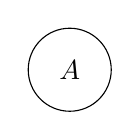
\begin{tikzpicture}
                \draw (0, 0) circle (1.5em) node {$A$};
            \end{tikzpicture}
            \\投出正面:$\Gh_1$
        \end{column}
        \begin{column}{0.5\textwidth}
            \centering
            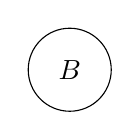
\begin{tikzpicture}
                \draw (0, 0) circle (1.5em) node {$B$};
            \end{tikzpicture}
            \\投出正面:$\Gh_2$
        \end{column}
    \end{columns}
    
    \pause

    \bigskip

    每轮投掷 $10$ 次,结果如下:

    \begin{table}
        \begin{tabular}{c|c|c|c|c|c}
            使用的硬币 & $B$ & $A$ & $A$ & $B$ & $A$ \\\hline
            投掷结果 & $5$ 正 $5$ 反 & $9$ 正 $1$ 反 & $8$ 正 $2$ 反 & $4$ 正 $6$ 反 & $7$ 正 $3$ 反
        \end{tabular}
    \end{table}

    \bigskip

    如何估计 $\Gh_1$ 和 $\Gh_2$?

\end{frame}

\begin{frame}
    \frametitle{投硬币实验}

    \begin{table}
        \begin{tabular}{c|c|c|c|c|c}
            使用的硬币 & $B$ & $A$ & $A$ & $B$ & $A$ \\\hline
            投掷结果 & $5$ 正 $5$ 反 & $9$ 正 $1$ 反 & $8$ 正 $2$ 反 & $4$ 正 $6$ 反 & $7$ 正 $3$ 反
        \end{tabular}
    \end{table}

    \bigskip

    分别用硬币为 $A$ 和 $B$ 的样本求 $\Gh_1$ 和 $\Gh_2$ 的最大似然估计。以 $A$ 为例,设 $X$ 为一次实验中出现正面的个数:

    \begin{itemize}
        \item $X \sim B(10, \Gh_1)$
        \item $X_1 = 9, X_2 = 8, X_3 = 7$
        \item 极大似然估计为 $\hat{\Gh_1} = \frac{\overline{X}}{10} = 0.8$
    \end{itemize}

\end{frame}

\begin{frame}
    \frametitle{投硬币实验}

    如果不知道每次使用的硬币怎么办?

    \begin{table}
        \begin{tabular}{c|c|c|c|c|c}
            使用的硬币 & ? & ? & ? & ? & ? \\\hline
            投掷结果 & $5$ 正 $5$ 反 & $9$ 正 $1$ 反 & $8$ 正 $2$ 反 & $4$ 正 $6$ 反 & $7$ 正 $3$ 反
        \end{tabular}
    \end{table}

\end{frame}

\end{document}